Long short-term memory networks are very similar to recurrent neural networks, but they address the issue of gradient approximation by introducing memory cells and a cell state \citep{hochreiter1997long}. A visualization of these networks is shown in Figure \ref{fig:LSTM}. The cell state acts as the "long term" memory, making use of all previous information. The only increase that can occur within the cell state is additive, which limits the impact of long-term dependencies that caused issues within RNNs. The memory cells act as the "short term" memory, making use of mostly the current input and previous output.

\begin{figure}[ht]
    \centering
    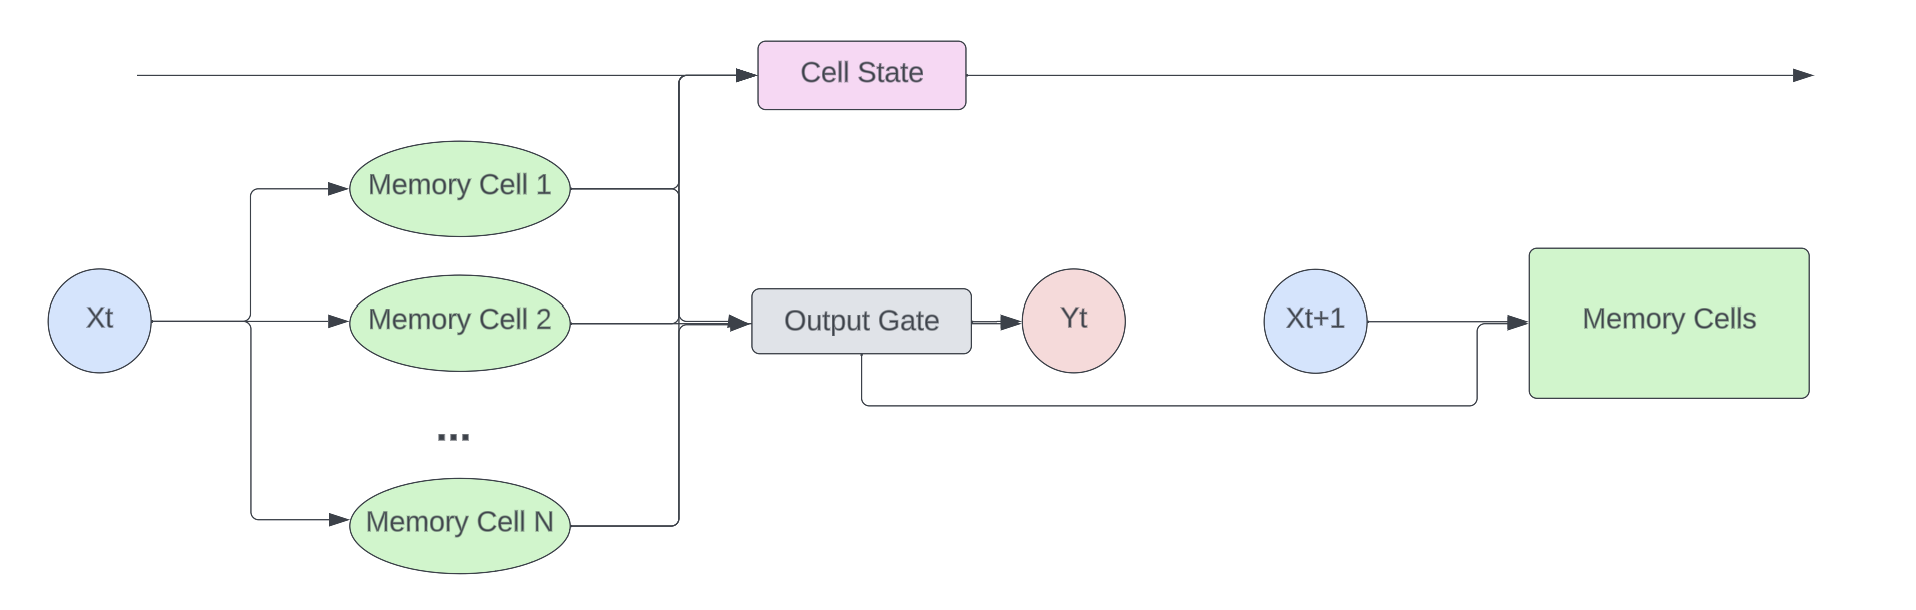
\includegraphics[width=0.8\linewidth]{"Figures/LSTM_Architecture.png"}
    \caption{A visualization of long short-term memory networks.}
    \label{fig:LSTM}
\end{figure}

\begin{figure}[ht]
    \centering
    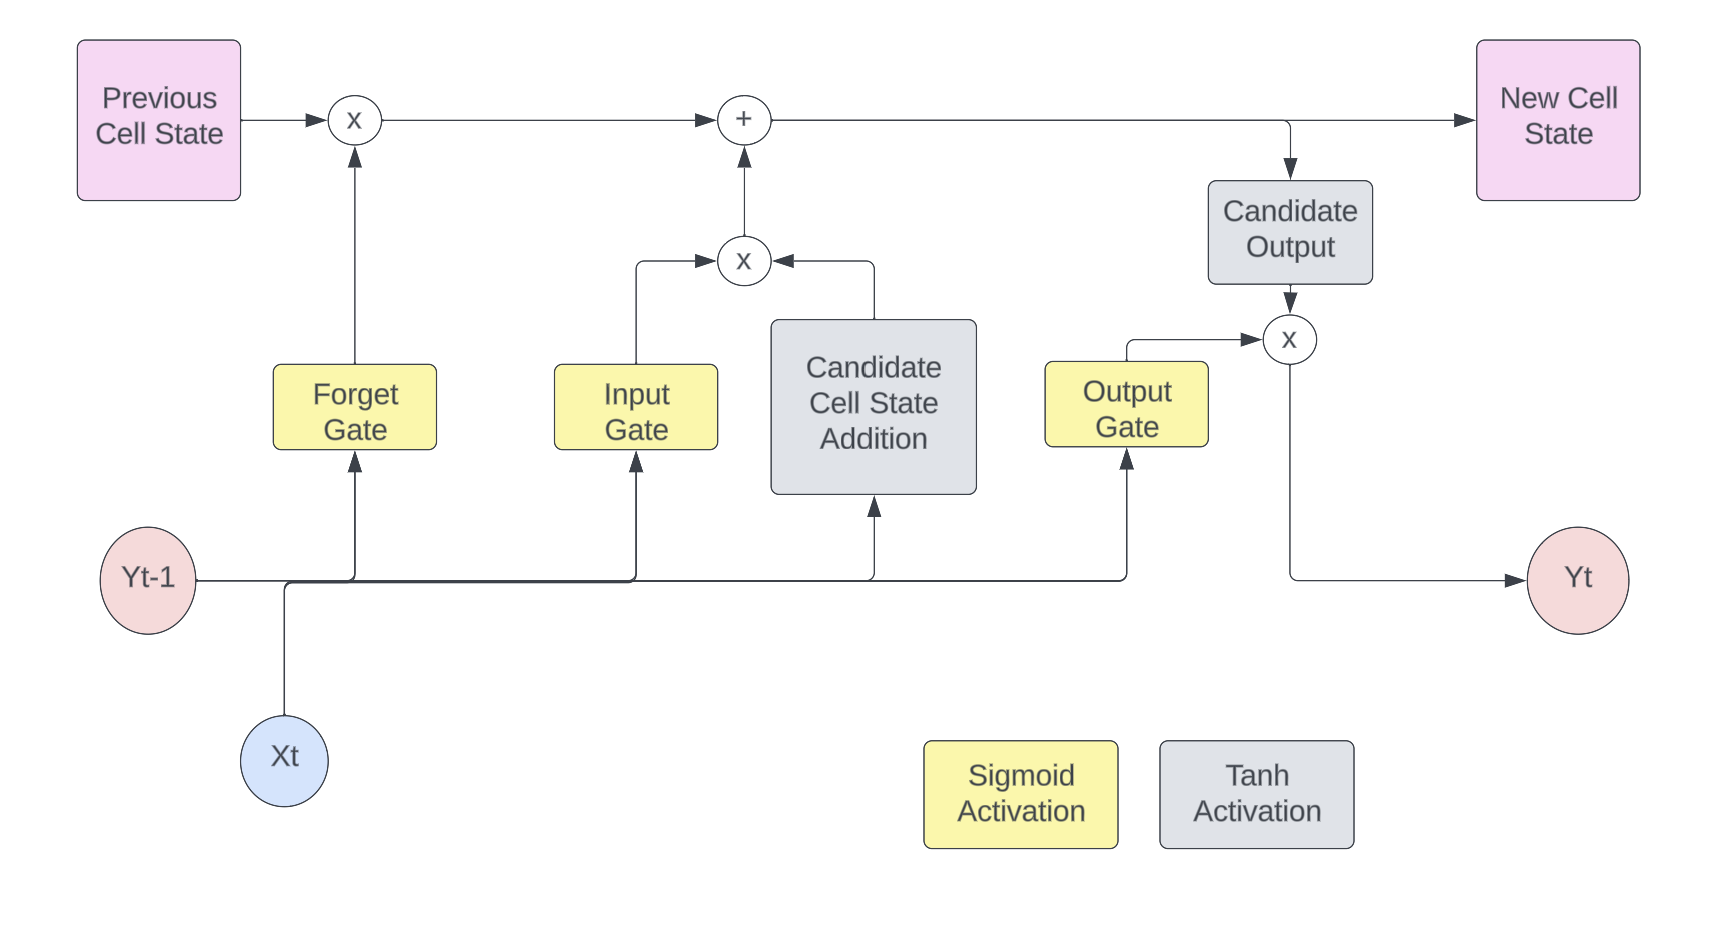
\includegraphics[width=0.6\linewidth]{"Figures/LSTM_Memory_Cell.png"}
    \caption{A visualization of the memory cells in LSTMs.}
    \label{fig:MemoryCells}
\end{figure}

The memory cells are more involved than the typical hidden states of RNNs (see Figure \ref{fig:MemoryCells}). The current input $x_t$ and previous output $y_{t-1}$ are used in more ways than simply getting the next prediction. The "forget gate" determines what percentage of the previous cell state is remembered. By using a sigmoid activation function, the forget gate value will be between 0 and 1. The cell state is then modified based on the candidate cell state addition, which is then multiplied by the input gate value. This gate acts similarly to the forget gate in the sense that it determines what percentage of the candidate cell state addition is actually added to the cell state. Finally, the cell state is fed into a hyperbolic tangent activation and multiplied by the output gate to determine that final output value $y_t$.

Mathematically, the memory cell can be written in notation used previously (adapted from \cite{understandinglstm}). The forget gate $f_t$ makes use of a sigmoid activation and has its own corresponding weights and bias, denoted $W_f$ and $b_f$, respectively.
\begin{equation*}
    f_t = \sigma[W_f(y_{t-1}, x_t) + b_f] 
\end{equation*}
The input gate $i_t$ functions similarly, with the notation of a subscript $i$.
\begin{equation*}
    i_t = \sigma[W_i(y_{t-1}, x_t) + b_i] 
\end{equation*}
The new candidate values $\tilde{C_t}$ to be added to the cell state use a hyperbolic tangent activation with the subscript $c$ on the weights and bias.
\begin{equation*}
    \tilde{C_t} = tanh[W_c(y_{t-1}, x_t) + b_c]
\end{equation*}
The updated cell state $C_t$ is the product of the forget gate $f_t$ and the previous cell state $C_{t-1}$ plus the new candidate cell state values $C_{t}$ multiplied by the input gate $i_t$.
\begin{equation*}
    C_t = f_t\cdot C_{t-1} + i_t\cdot \tilde{C_t}
\end{equation*}
Similar to previously mentioned gates, the output gate $o_t$ uses a sigmoid activation with the subscript $o$ on the weights and bias.
\begin{equation*}
    o_t = \sigma[W_o(y_{t-1}, x_t) + b_o]
\end{equation*}
The output value $y_t$ is calculated as a proportion (determined by the output gate) of the new cell state.
\begin{equation*}
    y_t = o_t\cdot tanh[C_t]
\end{equation*}
